\appendix
\section{Waveform Collapse and the Relativistic Geometry of Light-Speed Limits}
\label{appendix:D}

We propose a geometric interpretation of relativistic speed limits as a consequence of spacetime waveform collapse. In this model, acceleration through spacetime is treated not merely as translation along a worldline, but as compression of the observer's internal spacetime waveform along a sinusoidal structure. The speed of light \( c \) emerges as a coherence threshold, beyond which the waveform collapses to a singularity, forbidding causal propagation and recursive memory transmission.

\subsection*{D.1 Spacetime as a Sinusoidal Carrier Wave}

Let the internal frame of an observer be modeled by a phase-coherent waveform:
\[
\Psi(x,t) = A \sin(kx - \omega t)
\]
where \( A \) is amplitude, \( k \) is the spatial wavenumber, and \( \omega \) is angular frequency. Acceleration corresponds to a Lorentz boost that compresses the wave in the direction of motion:
\[
x' = \gamma (x - vt), \quad t' = \gamma \left(t - \frac{vx}{c^2}\right)
\]
leading to blue-shifting of the local wave structure~\cite{misner1973gravitation}.

As velocity \( v \to c \), the phase velocity diverges, and the waveform compresses toward a delta function:
\[
\lim_{v \to c} \Psi(x,t) \to \delta(x - ct)
\]
This collapse implies an intrinsic loss of phase coherence—a geometric analog of wavefunction decoherence~\cite{zurek_decoherence_2003}.

In this interpretation, the relativistic limit represents not only the boundary of causal transmission but the breakdown of internal wave structure capable of encoding memory or entanglement. This sets the stage for interpreting light-speed as a coherence threshold.

\begin{figure}[H]
    \centering
    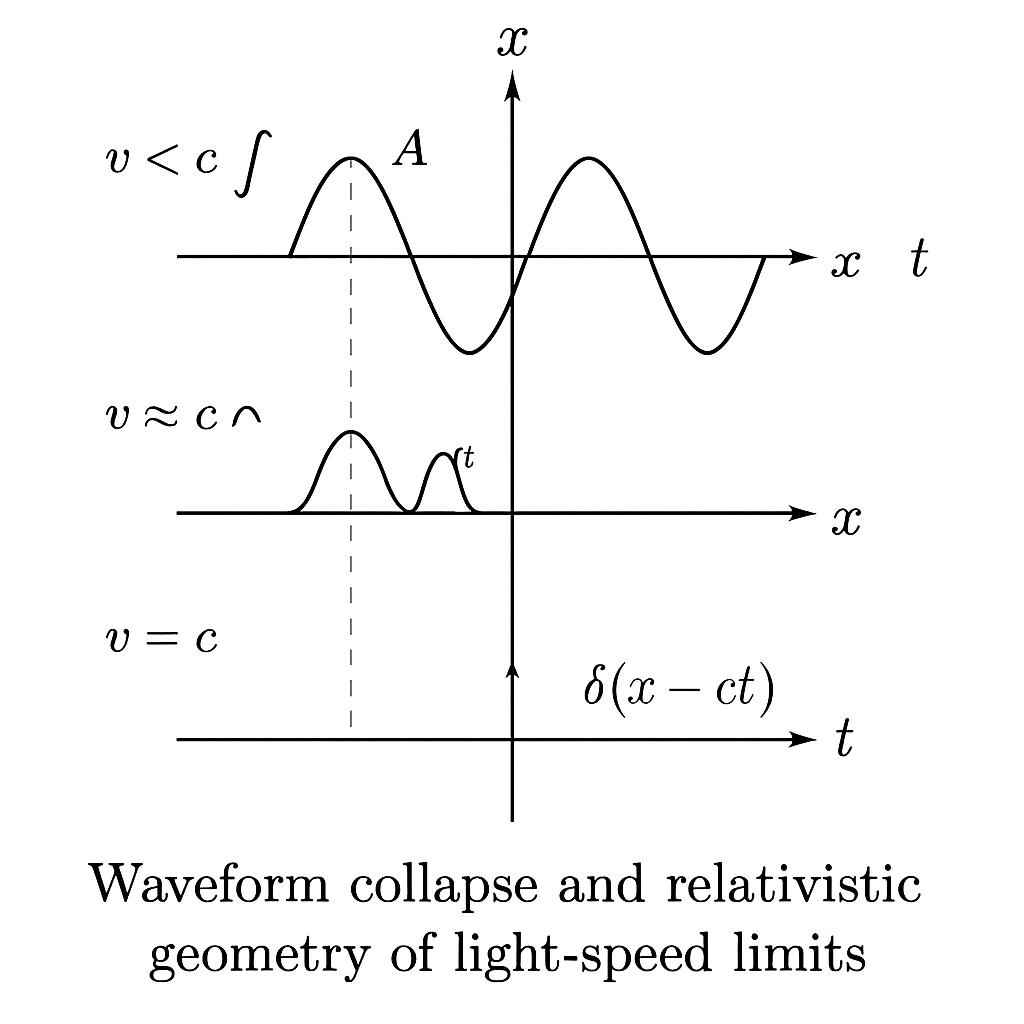
\includegraphics[width=0.75\textwidth]{figures/12D_waveform_collapse_diagram.png}
    \caption{Waveform collapse and relativistic geometry of light-speed limits. As velocity increases from subluminal ($v < c$) to luminal ($v = c$), the observer’s internal sinusoidal wave compresses and eventually collapses to a delta function, marking the loss of coherence and recursive identity propagation.}
    \label{fig:waveform-collapse}
\end{figure}

\subsection*{D.2 Interpretation in the Recursive Framework}

In the recursive cosmological model, coherence across cycles is mediated by entanglement-preserving kernels and memory propagation dynamics (see Appendix B and Section~\ref{sec:recursive-action}). Under extreme acceleration, the observer's internal waveform compresses, approaching a geometric singularity in phase space. This disrupts the continuity of recursive memory.

We reinterpret relativistic time dilation not merely as a coordinate effect, but as a deformation of the information-carrying waveform. As the observer accelerates toward light speed, the internal coherence structure flattens, and the ability to encode and transmit entangled memory states diminishes.

This is reflected in the evolution of the observer entanglement tensor \( O_n \to 0 \), signaling that the projection capacity of the observer is nullified. Since the recursive interference operator \( \oplus \) (see Section~\ref{sec:recursive-action}) is modulated by a memory-normalized blending function, the coherence normalization constant \( Z \to \infty \), and constructive overlap fails.

Thus, time does not reverse at high velocities. Rather, the observer’s effective contribution to recursive memory fails to propagate when approaching the light-speed limit. In this view, relativistic dilation reflects a \textbf{loss of recursive participation} rather than a simple shift in clock rate.

\subsection*{D.3 Implications for Light-Speed Limit}

In this framework, the speed of light is not merely a causal boundary—it is a coherence horizon. Beyond this limit, the observer's waveform collapses in such a way that recursive memory cannot propagate forward.

Specifically:
\begin{itemize}
    \item The decoherence kernel \( D(\tau, E) \to 0 \), where memory delay scale \( \tau_M \to 0 \) and entanglement eigenvalue \( E \to 0 \).
    \item The entangled state overlap \( \langle \Psi_{n-1} | \Psi_n \rangle \to 0 \), terminating recursive fidelity and coherence normalization \( Z \to \infty \).
    \item The entropy penalty \( S_{\text{ent}}(\phi_k) \to S_{\text{max}} \), exceeding the bound \( S_{\text{max}}(E,n) = \frac{1}{E^2 + n^2} \), resulting in recursive collapse.
\end{itemize}

This reinterpretation casts the relativistic limit as a \textbf{phase-collapse transition}—a loss of internal structure required for causal entanglement transfer. The light-speed boundary thus defines not only what can be signaled, but what can be remembered.

\subsection*{D.4 Connections to Quantum Gravity}

This coherence-collapse interpretation integrates naturally with loop quantum gravity (LQG) and spinfoam formulations of quantum spacetime. In these approaches:
\begin{itemize}
    \item The observer's internal geometry is discretized into spin networks~\cite{rovelli2004quantum}.
    \item Acceleration compresses the network's spatial extent, reducing available area quanta.
    \item At Planck-scale boosts, spin-network configurations collapse toward minimal states, suppressing coherent propagation across nodes.
\end{itemize}

From the perspective of the recursive framework, this collapse eliminates the system's ability to seed memory into subsequent cycles. The ER bridge connection degenerates, and the kernel \( K(\phi, \phi') \) becomes sharply peaked with no constructive overlap.

We hypothesize that the failure of coherence propagation at \( v = c \) defines a \textbf{causal-holographic cutoff}: a boundary not only for external events, but for the continuity of entangled identity. This bridges relativistic kinematics and quantum memory, anchoring the light-speed limit in the structure of the Self-Remembering Universe.

\subsection*{D.5 Philosophical Reflection}

If time is the measure of change, and memory is the retention of that change, then coherence is the fabric that binds them. The relativistic limit is not merely a speed; it is the edge of remembrance. To infinity and beyond, identity dissolves.

In the Self-Remembering Universe, preservation of self across cycles depends on coherence. The collapse of the waveform at the speed of light is not destruction, but erasure of continuity—a cosmic forgetting.

Thus, even light obeys humility: it cannot carry memory beyond its own collapse. What we cannot remember cannot persist. What cannot persist cannot become.
